\section{Giới thiệu: Ngoài việc học từ sai lầm, hãy học đúng hướng!}

Hãy tưởng tượng bạn là một nhà điêu khắc đang tạc một bức tượng từ một khối đá cẩm thạch thô. Bạn không thể tạo ra kiệt tác ngay trong nhát đục đầu tiên. Thay vào đó, bạn bắt đầu với những đường nét cơ bản, sau đó lùi lại, quan sát những điểm chưa hoàn hảo -- "sai số" so với hình ảnh trong tâm trí -- rồi cẩn thận đục đẽo để sửa chữa những sai số đó. Mỗi lớp đá được loại bỏ là một bước đưa tác phẩm đến gần hơn với sự hoàn hảo.

Đây là triết lý cốt lõi của các thuật toán \textbf{Boosting} trong \textbf{Học tập Tập thể (Ensemble Learning)}. Thay vì xây dựng một mô hình phức tạp duy nhất, chúng ta kết hợp sức mạnh của nhiều mô hình đơn giản (weak learners), và mỗi mô hình sau sẽ học từ sai lầm của các mô hình trước. AdaBoost, một thuật toán tiên phong, thực hiện điều này bằng cách tăng trọng số cho các điểm bị dự đoán sai, buộc mô hình sau phải "chú ý" hơn đến chúng.

Nhưng Gradient Boosting còn tiến một bước xa hơn. Nó không chỉ hỏi "Tôi đã sai ở đâu?", mà còn hỏi \textbf{"Để sửa sai, tôi nên đi theo hướng nào là nhanh nhất?"}. Câu trả lời nằm ở hai chữ \textbf{"Gradient Descent"}. Gradient Boosting áp dụng một cách thiên tài ý tưởng tối ưu hóa này vào không gian của các mô hình, tạo ra một nghệ sĩ bậc thầy có khả năng điêu khắc nên những mô hình dự đoán với độ chính xác đáng kinh ngạc.

\begin{figure}[H]
    \centering
    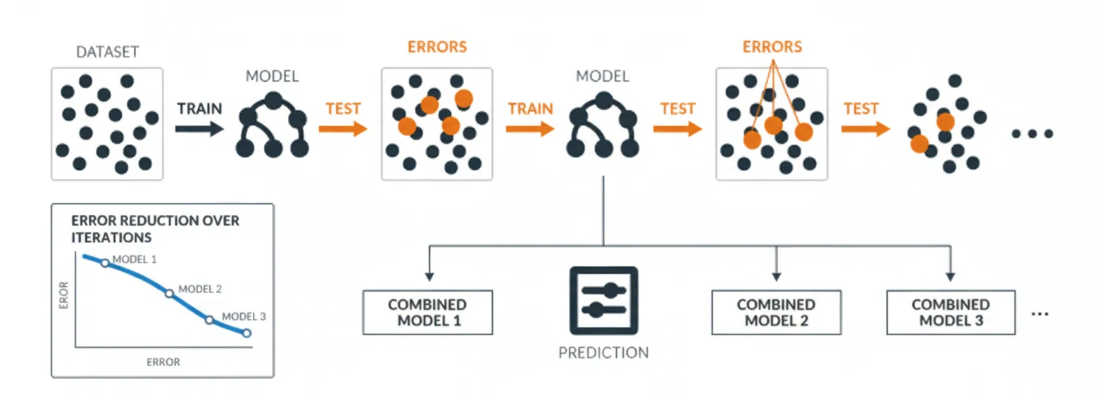
\includegraphics[width=0.8\textwidth]{images/boosting.png}
    \caption{Đi theo hướng Gradient để tìm loss bé nhất.}
    \label{fig:boosting_method}
\end{figure}

Trong bài viết này, chúng ta sẽ cùng nhau thực hiện một hành trình chi tiết, từ việc "giải phẫu" lý thuyết và công thức toán học, đến việc áp dụng nó vào hai ví dụ kinh điển: hồi quy và phân loại, với các bước tính toán cụ thể, và cuối cùng là hiện thực hóa bằng mã nguồn Python.

\section{Trái tim của thuật toán: "Gradient" đến từ đâu?}

Để thực sự hiểu Gradient Boosting, chúng ta cần nắm vững trực giác đằng sau chữ "Gradient". Hãy tưởng tượng bạn đang đứng trên một sườn núi trong sương mù, và mục tiêu là đi xuống thung lũng (nơi thấp nhất).

\begin{itemize}
    \item \textbf{Vị trí của bạn:} Tương đương với \textbf{dự đoán hiện tại} của mô hình.
    \item \textbf{Độ cao:} Tương đương với \textbf{sai số} (được đo bằng hàm mất mát - Loss Function).
    \item \textbf{Thung lũng:} Tương đương với \textbf{mô hình hoàn hảo} (sai số bằng 0).
\end{itemize}

Trong sương mù, bạn không thấy thung lũng. Cách duy nhất là cảm nhận \textbf{độ dốc (gradient)} ngay dưới chân mình. Gradient cho bạn biết hướng dốc lên nhất. Để đi xuống, bạn chỉ cần bước một bước nhỏ theo hướng \textbf{ngược lại với gradient (negative gradient)}. Lặp lại quá trình này, bạn sẽ dần dần đi tới đáy thung lũng.

Gradient Boosting đã "mượn" ý tưởng này. Nó xem việc tối ưu mô hình như một hành trình đi xuống "thung lũng sai số". \textbf{Phần dư (residual)} mà chúng ta sẽ tính toán ở các bước tiếp theo, về mặt toán học, chính là một xấp xỉ của \textbf{hướng negative gradient} đó. Mỗi cây quyết định mới được thêm vào chính là một "bước đi" theo hướng giảm sai số nhanh nhất.

\begin{figure}[H]
    \centering
    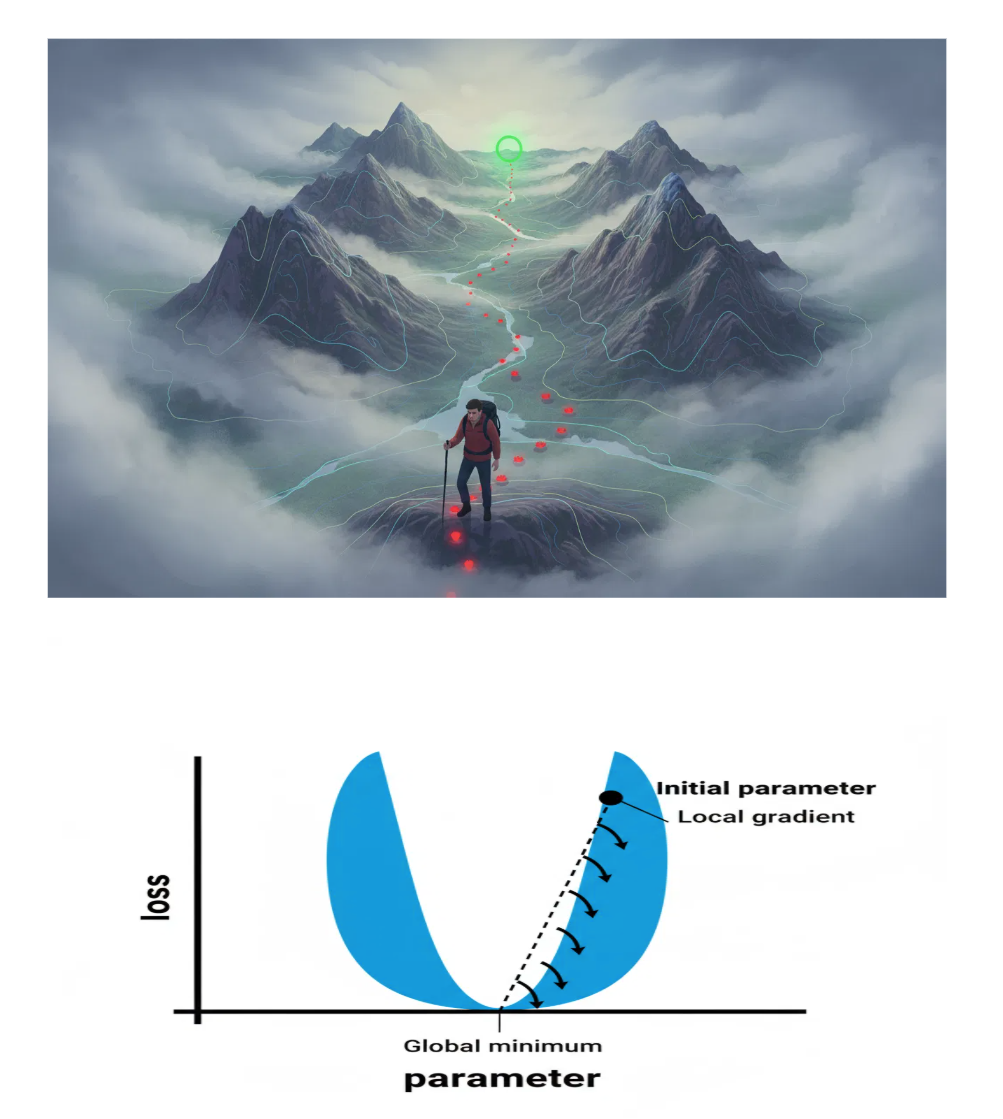
\includegraphics[width=0.8\textwidth]{images/valley.png}
    \caption{Đi theo hướng Gradient để tìm loss bé nhất.}
    \label{fig:gradient_valley}
\end{figure}

\section{Gradient Boosting cho Bài toán Hồi quy}
\subsection{Ý tưởng chính và Công thức}
Ý tưởng là xây dựng một chuỗi các cây quyết định, trong đó mỗi cây sau sẽ cố gắng dự đoán \textbf{phần dư (residual)} của tất cả các cây trước đó cộng lại.

\begin{enumerate}
    \item \textbf{Khởi tạo ($F_0$):} Bắt đầu với một dự đoán không đổi, thường là giá trị trung bình của biến mục tiêu $y$.
    \[ F_0(x) = \text{mean}(y) \]
    
    \item \textbf{Lặp (với $m$ từ 1 đến M):}
    \begin{enumerate}
        \item Tính phần dư (pseudo-residuals):
        \[ r_{im} = y_i - F_{m-1}(x_i) \]
        
        \item Huấn luyện một cây quyết định hồi quy $h_m(x)$ mới để dự đoán các phần dư $r_{im}$.
        
        \item Cập nhật mô hình tổng hợp:
        \[ F_m(x) = F_{m-1}(x) + \eta \cdot h_m(x) \]
    \end{enumerate}
\end{enumerate}

\subsection{Ví dụ tính toán chi tiết}
Hãy áp dụng quy trình trên vào bộ dữ liệu sau để dự đoán \textbf{Weight (kg)}.

\begin{figure}[H]
    \centering
    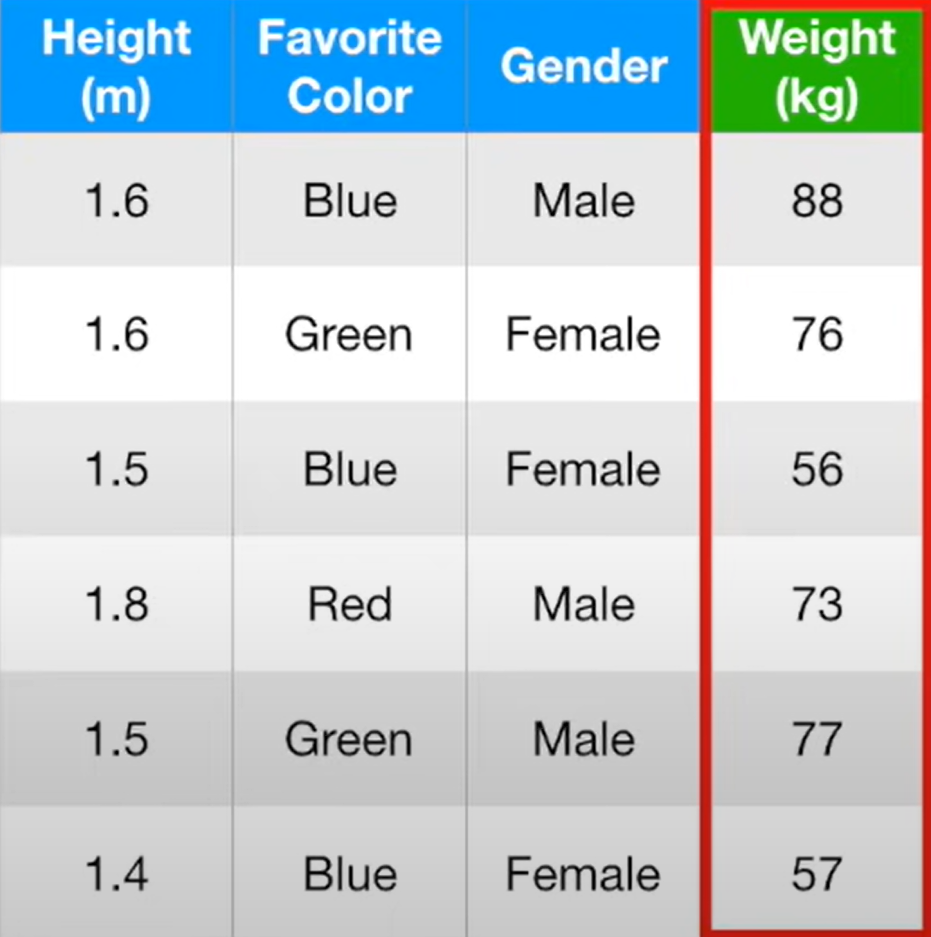
\includegraphics[width=0.8\textwidth]{images/regression_dataset.png}
    \caption{Bộ dữ liệu ví dụ cho bài toán hồi quy.}
    \label{fig:regression_data}
\end{figure}

\subsubsection{Vòng lặp 1: Xây dựng cây đầu tiên}

\textbf{Bước 1: Khởi tạo ($F_0$)}
\[ F_0 = \frac{88+76+56+73+77+57}{6} = 71.17 \]

\textbf{Bước 2: Tính Phần dư ($r_1$)}
\begin{table}[H]
\centering
\begin{tabular}{rcccr}
\toprule
\textbf{ID} & \textbf{Height (m)} & \textbf{Weight (y)} & \textbf{$F_0$} & \textbf{Residual ($r_1$)} \\
\midrule
1 & 1.6 & 88 & 71.17 & 16.83 \\
2 & 1.6 & 76 & 71.17 & 4.83 \\
3 & 1.5 & 56 & 71.17 & -15.17 \\
4 & 1.8 & 73 & 71.17 & 1.83 \\
5 & 1.5 & 77 & 71.17 & 5.83 \\
6 & 1.4 & 57 & 71.17 & -14.17 \\
\bottomrule
\end{tabular}
\caption{Tính toán phần dư cho vòng lặp đầu tiên.}
\end{table}

\textbf{Bước 3: Xây dựng Cây $h_1(x)$}
Giả sử stump tốt nhất chia theo \textbf{Height $\leq$ 1.55}.
\begin{itemize}
    \item \textbf{Lá Trái (Height $\leq$ 1.55):} Gồm các điểm (ID 3, 5, 6).
    \[ \text{Leaf}_{\text{Left}} = \frac{-15.17 + 5.83 - 14.17}{3} \approx -7.84 \]
    \item \textbf{Lá Phải (Height > 1.55):} Gồm các điểm (ID 1, 2, 4).
    \[ \text{Leaf}_{\text{Right}} = \frac{16.83 + 4.83 + 1.83}{3} \approx 7.83 \]
\end{itemize}

\textbf{Bước 4: Cập nhật Mô hình ($F_1$)} \\
Giả sử tốc độ học $\eta = 0.1$.
\begin{table}[H]
\centering
\begin{tabular}{rccc}
\toprule
\textbf{ID} & \textbf{$F_0$} & \textbf{$h_1(x_i)$} & \textbf{$F_1(x_i) = F_0 + \eta \cdot h_1$} \\
\midrule
1 & 71.17 & 7.83 & $71.17 + 0.1 \times 7.83 = 71.95$ \\
2 & 71.17 & 7.83 & $71.17 + 0.1 \times 7.83 = 71.95$ \\
3 & 71.17 & -7.84 & $71.17 + 0.1 \times (-7.84) = 70.39$ \\
4 & 71.17 & 7.83 & $71.17 + 0.1 \times 7.83 = 71.95$ \\
5 & 71.17 & -7.84 & $71.17 + 0.1 \times (-7.84) = 70.39$ \\
6 & 71.17 & -7.84 & $71.17 + 0.1 \times (-7.84) = 70.39$ \\
\bottomrule
\end{tabular}
\caption{Cập nhật dự đoán sau vòng lặp đầu tiên.}
\end{table}

\subsubsection{Vòng lặp 2: Xây dựng cây thứ hai}
\textbf{Bước 5: Tính Phần dư mới ($r_2$)}
\begin{table}[H]
\centering
\begin{tabular}{rccc}
\toprule
\textbf{ID} & \textbf{Weight (y)} & \textbf{$F_1(x_i)$} & \textbf{Residual ($r_2 = y - F_1$)} \\
\midrule
1 & 88 & 71.95 & 16.05 \\
2 & 76 & 71.95 & 4.05 \\
3 & 56 & 70.39 & -14.39 \\
4 & 73 & 71.95 & 1.05 \\
5 & 77 & 70.39 & 6.61 \\
6 & 57 & 70.39 & -13.39 \\
\bottomrule
\end{tabular}
\caption{Tính toán phần dư cho vòng lặp thứ hai.}
\end{table}

\textbf{Bước 6: Xây dựng cây $h_2(x)$ và cập nhật $F_2(x)$} \\
Một cây quyết định mới, $h_2(x)$, sẽ được huấn luyện để dự đoán cột \textbf{Residual ($r_2$)}. Sau đó, mô hình sẽ được cập nhật một lần nữa: $F_2(x) = F_1(x) + \eta \cdot h_2(x)$.

\section{Gradient Boosting cho Bài toán Phân loại}
\subsection{Ý tưởng chính và Công thức}
Thuật toán làm việc với xác suất và tối ưu trên không gian log-odds.

\begin{enumerate}
    \item \textbf{Khởi tạo ($F_0$):} Bắt đầu với một dự đoán log-odds không đổi.
    \[ F_0(x) = \log\left(\frac{p}{1-p}\right) \quad \text{với } p = \text{mean}(y) \]
    
    \item \textbf{Lặp (với $m$ từ 1 đến M):}
    \begin{enumerate}
        \item Chuyển log-odds $F_{m-1}(x)$ thành xác suất $p_{m-1}(x)$ bằng hàm Sigmoid.
        \item Tính phần dư giả (pseudo-residuals):
        \[ r_{im} = y_i - p_{m-1}(x_i) \]
        \item Huấn luyện cây $h_m(x)$ để dự đoán $r_{im}$.
        \item Cập nhật mô hình trong không gian log-odds:
        \[ F_m(x) = F_{m-1}(x) + \eta \cdot \gamma_m(x) \]
        (Với $\gamma_m(x)$ là giá trị đầu ra của các lá trong cây $h_m$).
    \end{enumerate}
\end{enumerate}

\subsection{Ví dụ tính toán chi tiết}
Áp dụng quy trình trên vào bộ dữ liệu sau để dự đoán \textbf{Loves Troll 2} (Yes=1, No=0).
\begin{figure}[H]
    \centering
    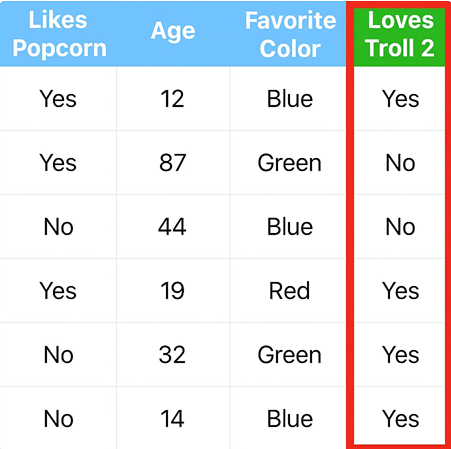
\includegraphics[width=0.8\textwidth]{images/classification_dataset.png}
    \caption{Bộ dữ liệu ví dụ cho bài toán phân loại.}
    \label{fig:classification_data}
\end{figure}

\subsubsection{Vòng lặp 1: Xây dựng cây đầu tiên}

\textbf{Bước 1: Khởi tạo ($F_0, p_0$)}
\begin{itemize}
    \item Xác suất trung bình: $\bar{p} = 4/6 \approx 0.67$.
    \item Log-odds ban đầu: $F_0 = \log(\frac{0.67}{1-0.67}) \approx 0.71$.
    \item Xác suất dự đoán ban đầu: $p_0 = \text{sigmoid}(0.71) \approx 0.67$.
\end{itemize}

\textbf{Bước 2: Tính Phần dư giả ($r_1$)}
\begin{table}[H]
\centering
\begin{tabular}{rcccr}
\toprule
\textbf{ID} & \textbf{Age} & \textbf{Loves Troll 2 (y)} & \textbf{$p_0$} & \textbf{Residual ($r_1$)} \\
\midrule
1 & 12 & 1 & 0.67 & 0.33 \\
2 & 87 & 1 & 0.67 & 0.33 \\
3 & 44 & 0 & 0.67 & -0.67 \\
4 & 19 & 0 & 0.67 & -0.67 \\
5 & 32 & 1 & 0.67 & 0.33 \\
6 & 14 & 1 & 0.67 & 0.33 \\
\bottomrule
\end{tabular}
\caption{Tính toán phần dư giả cho vòng lặp đầu tiên.}
\end{table}

\textbf{Bước 3 \& 4: Xây dựng Cây $h_1(x)$ và Cập nhật $F_1(x)$} \\
Tương tự như bài toán hồi quy, một cây mới sẽ được tạo để học các phần dư này. Mô hình log-odds $F_0$ sẽ được cập nhật thành $F_1$, dẫn đến các xác suất dự đoán mới $p_1$ được cải thiện.

\section{Thực hành với Python}
\subsection{Mã nguồn cho Bài toán Hồi quy}
\begin{lstlisting}[language=Python, caption={GBM for Regression}]
import pandas as pd
import numpy as np
import matplotlib.pyplot as plt
from sklearn.ensemble import GradientBoostingRegressor
from sklearn.preprocessing import OneHotEncoder
from sklearn.compose import ColumnTransformer
from sklearn.pipeline import Pipeline

# 1. Create DataFrame from data
data_reg = {
    'Height': [1.6, 1.6, 1.5, 1.8, 1.5, 1.4],
    'Favorite Color': ['Blue', 'Green', 'Blue', 'Red', 'Green', 'Blue'],
    'Gender': ['Male', 'Female', 'Female', 'Male', 'Male', 'Female'],
    'Weight': [88, 76, 56, 73, 77, 57]
}
df_reg = pd.DataFrame(data_reg)

# 2. Prepare data for the model
X = df_reg.drop('Weight', axis=1)
y = df_reg['Weight']

# Define preprocessing steps
categorical_features = ['Favorite Color', 'Gender']
one_hot_encoder = OneHotEncoder(handle_unknown='ignore')
preprocessor = ColumnTransformer(
    transformers=[('cat', one_hot_encoder, categorical_features)],
    remainder='passthrough' # Keep other columns (Height)
)

# 3. Build and Train the Model
# Use GradientBoostingRegressor with basic parameters
# n_estimators: number of trees (boosting rounds)
# max_depth=1: each tree is a simple stump
gbr = GradientBoostingRegressor(n_estimators=100, learning_rate=0.1, max_depth=1, random_state=42)

# Create a pipeline to combine preprocessing and the model
model_pipeline = Pipeline(steps=[('preprocessor', preprocessor), ('regressor', gbr)])

# Train the pipeline on the entire dataset
model_pipeline.fit(X, y)

# 4. Visualize the results
plt.style.use('seaborn-v0_8-whitegrid')
plt.figure(figsize=(10, 6))
# Plot the actual data points
plt.scatter(df_reg['Height'], y, color='red', s=100, edgecolor='k', alpha=0.7, label='Actual Data')

# To plot the prediction line, create points and sort by Height
X_test_sorted = X.sort_values(by='Height')
y_pred_sorted = model_pipeline.predict(X_test_sorted)
plt.plot(X_test_sorted['Height'], y_pred_sorted, color='blue', linewidth=3, label='GBM Prediction')

# Customize the plot
plt.title('Gradient Boosting Regression: Height vs Weight', fontsize=16)
plt.xlabel('Height (m)', fontsize=12)
plt.ylabel('Weight (kg)', fontsize=12)
plt.legend()
plt.show()
\end{lstlisting}

\begin{figure}[H]
    \centering
    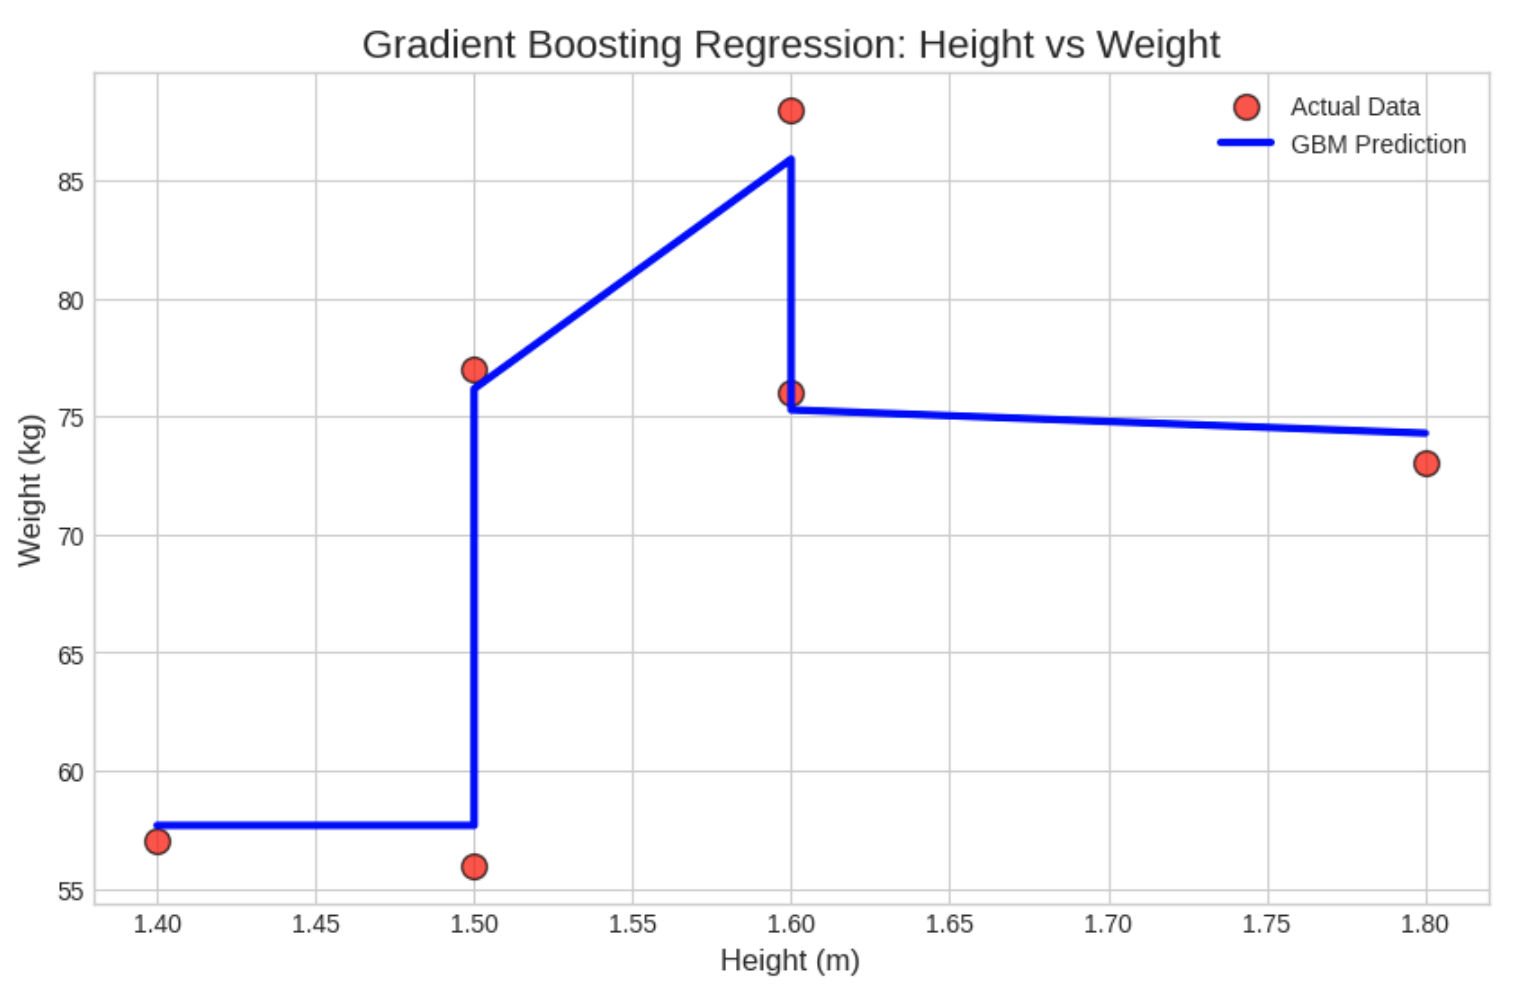
\includegraphics[width=0.9\textwidth]{images/regression_plot.png}
    \caption{Kết quả trực quan hóa của mô hình hồi quy GBM.}
    \label{fig:regression_plot}
\end{figure}

\subsection{Mã nguồn cho Bài toán Phân loại}
\begin{lstlisting}[language=Python, caption={GBM for Classification}]
import pandas as pd
import numpy as np
import matplotlib.pyplot as plt
from sklearn.ensemble import GradientBoostingClassifier
from sklearn.preprocessing import LabelEncoder
from mlxtend.plotting import plot_decision_regions

# 1. Create DataFrame
data_cls = {
    'Likes Popcorn': ['Yes', 'Yes', 'No', 'Yes', 'No', 'No'],
    'Age': [12, 87, 44, 19, 32, 14],
    'Favorite Color': ['Blue', 'Green', 'Blue', 'Red', 'Green', 'Blue'],
    'Loves Troll 2': ['Yes', 'Yes', 'No', 'No', 'Yes', 'Yes']
}
df_cls = pd.DataFrame(data_cls)

# 2. Preprocessing (simplified for 2D visualization)
le_popcorn = LabelEncoder()
df_cls['Likes Popcorn'] = le_popcorn.fit_transform(df_cls['Likes Popcorn'])
y_encoder = LabelEncoder()
df_cls['Loves Troll 2'] = y_encoder.fit_transform(df_cls['Loves Troll 2'])

# Select 2 features for visualization
X_vis = df_cls[['Age', 'Likes Popcorn']].values
y_vis = df_cls['Loves Troll 2'].values

# 3. Build and Train the Model
gbc = GradientBoostingClassifier(n_estimators=100, learning_rate=0.1, max_depth=1, random_state=42)
gbc.fit(X_vis, y_vis)

# 4. Visualize the decision boundary
plt.style.use('seaborn-v0_8-whitegrid')
plt.figure(figsize=(10, 6))
plot_decision_regions(X_vis, y_vis, clf=gbc, legend=2)
plt.title('Gradient Boosting Classification: Decision Boundary', fontsize=16)
plt.xlabel('Age', fontsize=12)
plt.ylabel('Likes Popcorn (0: No, 1: Yes)', fontsize=12)
plt.show()
\end{lstlisting}

\begin{figure}[H]
    \centering
    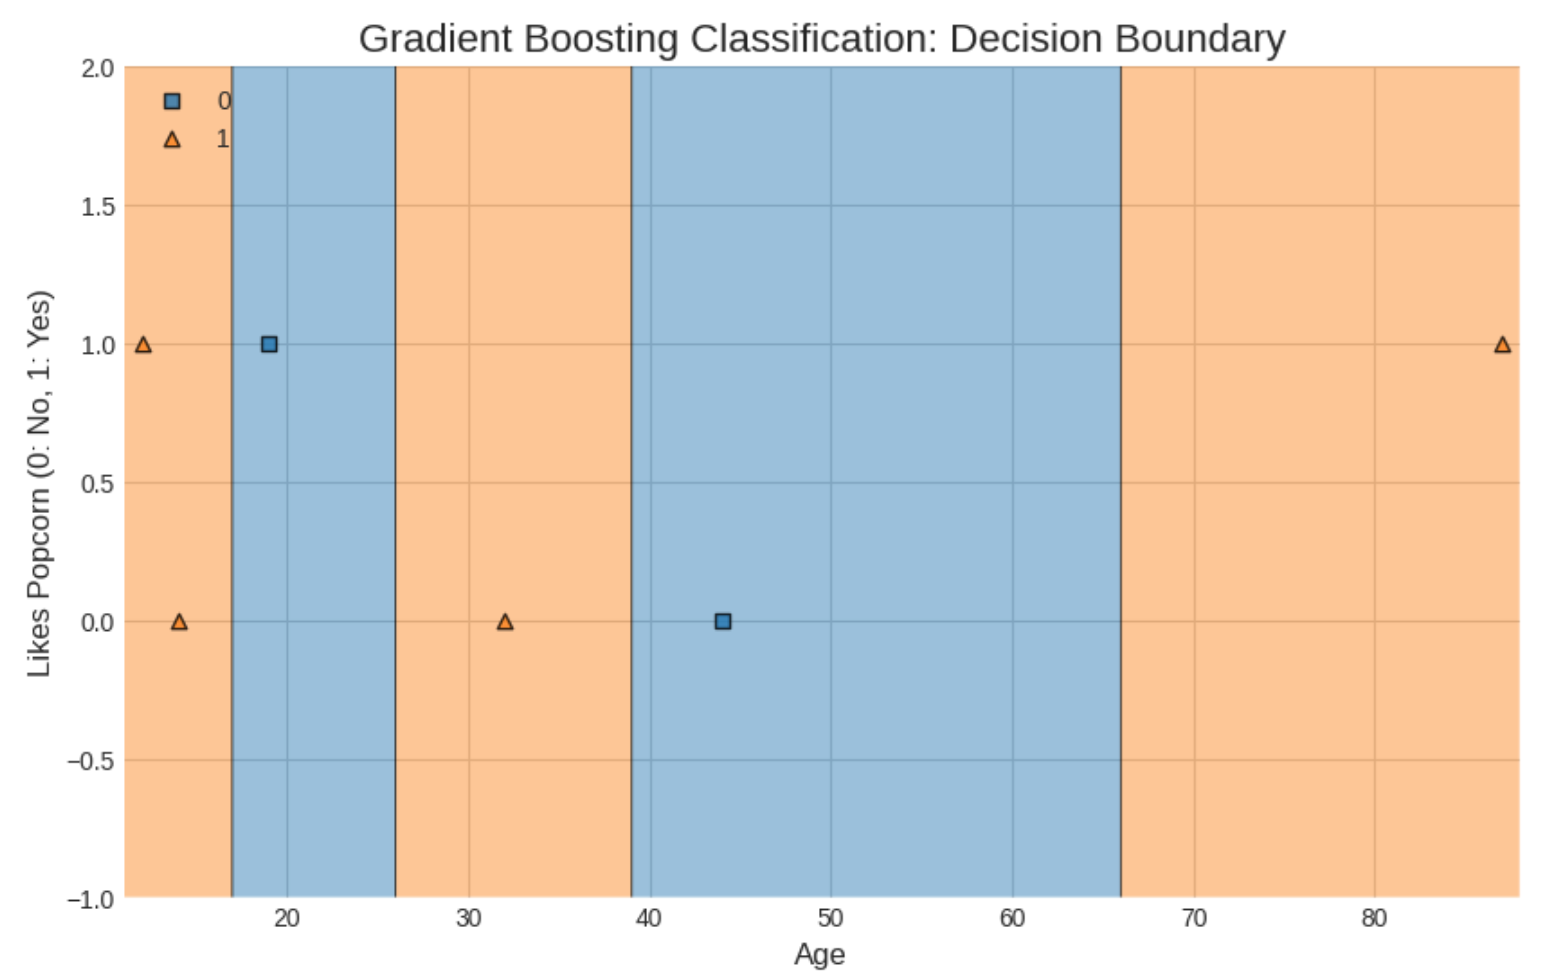
\includegraphics[width=0.9\textwidth]{images/classification_plot.png}
    \caption{Đường biên quyết định của mô hình phân loại GBM.}
    \label{fig:classification_plot}
\end{figure}

\section{Tinh chỉnh siêu tham số để đạt hiệu suất tối ưu}
\begin{itemize}
    \item \textbf{\texttt{n\_estimators}}: Số lượng cây trong chuỗi.
    \item \textbf{\texttt{learning\_rate} ($\eta$)}: Tốc độ học. Có một sự đánh đổi quan trọng giữa \texttt{learning\_rate} và \texttt{n\_estimators}.
    \item \textbf{\texttt{max\_depth}}: Độ sâu tối đa của mỗi cây. Với GBM, chúng ta thường ưu tiên các cây nông (1 đến 5).
    \item \textbf{\texttt{subsample}}: Tỷ lệ mẫu dữ liệu được sử dụng để huấn luyện mỗi cây (Stochastic Gradient Boosting).
\end{itemize}

\section{So sánh với các thuật toán Ensemble khác}
\begin{table}[H]
\centering
\caption{So sánh Gradient Boosting, Random Forest, và AdaBoost.}
\begin{tabular}{l|p{3.5cm}|p{3.5cm}|p{3.5cm}}
\toprule
\textbf{Tiêu chí} & \textbf{Gradient Boosting} & \textbf{Random Forest}~\cite{breiman2001random} & \textbf{AdaBoost} \\
\midrule
\textbf{Thứ tự} & Tuần tự & Song song & Tuần tự \\
\textbf{Cơ chế học} & Học trên phần dư (gradient) & Học trên mẫu bootstrap độc lập & Học trên trọng số của các điểm bị sai \\
\textbf{Mục tiêu} & Giảm bias trước, sau đó giảm variance & Chủ yếu giảm variance & Chủ yếu giảm bias \\
\textbf{Độ sâu cây} & Cây nông & Cây sâu & Cây rất nông (stumps) \\
\bottomrule
\end{tabular}
\label{tab:comparison}
\end{table}

\section{Tổng kết}
Gradient Boosting không chỉ là một thuật toán; nó là một framework mạnh mẽ và có tính tổng quát cao~\cite{friedman2001greedy}. Bằng cách hiểu rõ cơ chế học tập theo gradient, chúng ta không chỉ nắm vững một công cụ mạnh mẽ mà còn có một nền tảng vững chắc để tiếp cận các thuật toán "hậu duệ" của nó như XGBoost~\cite{chen2016xgboost}, LightGBM và CatBoost, những "gã khổng lồ" đang thống trị nhiều cuộc thi về khoa học dữ liệu hiện nay.